\documentclass[conference]{IEEEtran}
\IEEEoverridecommandlockouts
\usepackage{amsmath,amssymb}
\usepackage{graphicx}
\usepackage{booktabs}
\usepackage{array}
\usepackage{url}
\usepackage{cite}
\usepackage{balance}
\graphicspath{{figures/}}
\hyphenation{input-output inter-country supply-chain}

\title{Structural Centrality, Disruption Propagation, and Resilience in a Global Production Network: An Analysis of OECD ICIO 2022}

\author{\IEEEauthorblockN{Group [Number] -- [Member Names]}
\IEEEauthorblockA{SC452: Processes on Networks\\\textit{Institution / Department}}}

\begin{document}
\maketitle

\begin{abstract}
Global production depends on inter-industry input flows that connect suppliers and buyers across national boundaries. A disruption at one country--industry node may therefore affect downstream production through several layers of dependencies. This project constructs a directed, weighted network from the 2022 OECD Inter-Country Input-Output (ICIO) table and studies how its structure relates to simulated disruption propagation. The raw network contains 4,050 country--industry nodes and 10.17 million positive off-diagonal links, although the measured density changes sharply when very small flows are excluded. For tractable dynamics, we aggregate the data into 1,053 country--sector nodes while preserving total flows and gross output. We compare an unweighted SIS process with a supplier-dependency-weighted SIS process, examine deterministic threshold cascades, and test equal-budget protection strategies. In 100-run experiments, targeted protection of high out-strength nodes reduced mean peak disruption and cumulative disrupted-share time more than random protection under our chosen assumptions. These are counterfactual stress tests, not forecasts of real economic losses.
\end{abstract}

\begin{IEEEkeywords}
production networks, input-output analysis, complex networks, SIS model, threshold cascade, centrality, resilience
\end{IEEEkeywords}

\section{Introduction}
The production of a good or service usually depends on inputs from other industries. A manufacturer may require electricity, metal products, transport, finance, and professional services; those suppliers in turn depend on other producers. This creates a network in which a local disruption can be transmitted indirectly. Work on production networks has shown that inter-sectoral connections can transmit sector-specific shocks and contribute to aggregate fluctuations [2]. Supply-chain risk has also been studied with epidemic-style models, where disruptions spread through supplier--buyer relationships [3].

Our project asks: \emph{Which structural properties of a real production network are associated with the greatest simulated propagation of a supplier disruption, and which simple protection strategy best limits that propagation under a fixed budget?} We do not attempt to forecast a real crisis. Instead, we use a public input-output table to build a reproducible network and compare explicit mathematical stress-test models.

The contributions of this course project are: (1) a structural analysis of the complete 2022 country--industry matrix; (2) a sensitivity check showing how binary topology depends on the minimum monetary flow treated as an edge; (3) an unweighted-versus-weighted SIS comparison and a separate nonlinear threshold-cascade experiment; and (4) an equal-budget comparison of random, out-strength-based, and PageRank-based protection. The difference between observed data and simulated behaviour is maintained throughout: the ICIO table records annual economic flows, not the timing or outcome of actual industry outages.

\begin{figure*}[t]
\centering
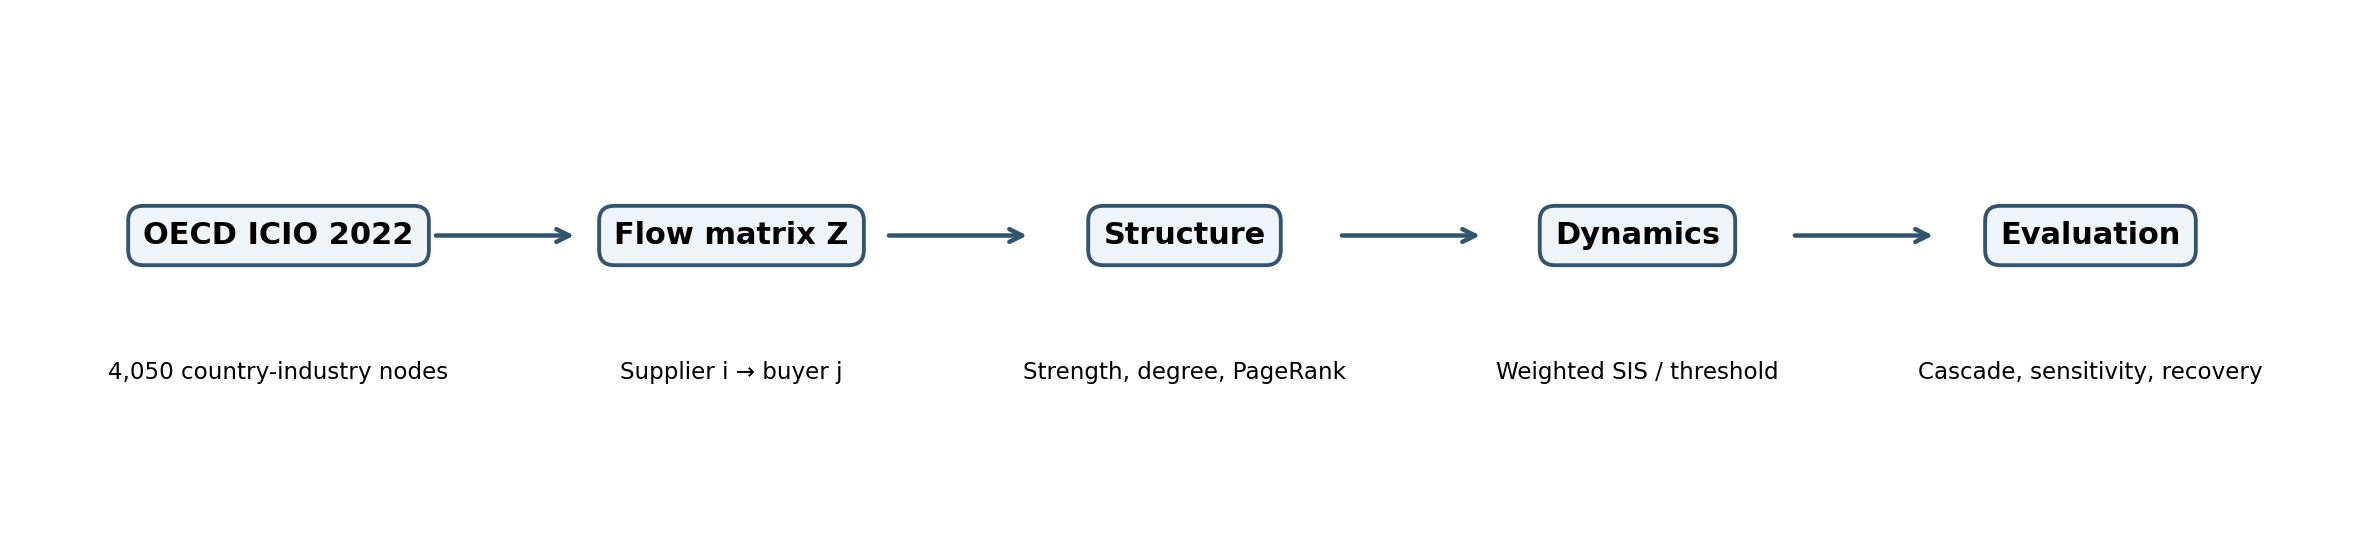
\includegraphics[width=0.96\textwidth]{analysis_pipeline.png}
\caption{Analysis pipeline developed from the raw 2022 ICIO table. Structural metrics are computed on the full network; repeated dynamics are run on the aggregated network.}
\label{fig:pipeline}
\end{figure*}

\section{Data and Network Construction}
\subsection{ICIO table}
We use the regular OECD ICIO 2025-edition dataset for the year 2022 [1]. The regular table covers 80 economies plus a Rest-of-the-World aggregate and 50 economic activities, giving $81\times 50=4{,}050$ country--industry nodes. Monetary entries are in millions of current U.S. dollars. The table includes intermediate flows, final-demand categories, and supporting output/value-added rows. Only the $4{,}050\times4{,}050$ intermediate-flow block is used to define the supply network; the gross-output vector is retained for weighting summary measures.

Let $Z_{ij}$ denote the value of intermediate inputs supplied by country--industry $i$ and used by country--industry $j$. We use the direction $i\rightarrow j$ to mean \emph{supplier to purchaser}. A positive off-diagonal entry defines an edge, with $Z_{ij}$ as its monetary weight. Exact self-links are excluded from graph degree and inter-node propagation, but the flow totals are retained when validating the input-output table and when computing total input denominators after sector aggregation.

\subsection{Structural measures}
The binary adjacency matrix is
\begin{equation}
A_{ij}=\begin{cases}1,&Z_{ij}>0,\ i\ne j,\\0,&\text{otherwise.}\end{cases}
\label{eq:adj}
\end{equation}
Out-degree and in-degree count distinct buyers and suppliers, respectively. Weighted out-strength and in-strength measure total supplied and purchased intermediate flows:
\begin{equation}
s_i^{\mathrm{out}}=\sum_j Z_{ij},\qquad s_j^{\mathrm{in}}=\sum_i Z_{ij},
\label{eq:strength}
\end{equation}
where the diagonal is omitted for graph metrics. Directed density is $m/[n(n-1)]$. We also calculate weak and strong components, weighted PageRank, and Spearman rank correlations between structural measures. A sensitivity analysis repeats the binary graph calculation after excluding flows below selected monetary thresholds. This check is important because even tiny positive transactions count as edges in the unthresholded graph.

\subsection{Aggregation for dynamic experiments}
Repeated stochastic simulation on the 4,050-node network is computationally more expensive and harder to interpret. We therefore map the 50 original activities into 13 broad sector groups, while retaining all 81 economy/region labels. This yields $81\times13=1{,}053$ country--sector nodes. Flows and output are summed into the corresponding groups. A conservation check confirms that aggregated total intermediate flows and aggregate gross output match the totals before aggregation to numerical precision (the code uses a relative-error tolerance of $10^{-8}$).

Aggregation combines some distinct industries and may hide within-group heterogeneity. For propagation, flows between distinct aggregate nodes form the links; flows that become internal to an aggregate are not used as external edges, but are retained in the purchasing node's total-input denominator for the threshold model. The model results should therefore be interpreted at the aggregated country--sector level.

\section{Dynamical Models}
\subsection{Dependency-weighted SIS process}
We adapt SIS epidemiology as an analogy for recurring supply disruption. Each aggregate node is either susceptible/operational, $I_j(t)=0$, or disrupted, $I_j(t)=1$. A disrupted node may recover and later be disrupted again. This is more suitable than a basic SIR process for a stress test in which nodes are not permanently removed after one event. SIS-style disruption modelling has prior precedent in supply-network research [3]; our aim is to compare simple variants on the ICIO network, not to claim the model family itself is new.

For the weighted model, define the off-diagonal technical-coefficient-like transmission weight
\begin{equation}
W_{ij}=\frac{Z^{\mathrm{cross}}_{ij}}{X_j},
\label{eq:weighted}
\end{equation}
where $X_j$ is the gross output of purchaser $j$ and $Z^{\mathrm{cross}}_{ij}$ is the flow from supplier $i$ to a distinct aggregate buyer $j$. This approximates the input-flow scale relative to buyer output; it is used here as a propagation weight, not as an estimated probability of failure. For the unweighted baseline, let $U_{ij}=A_{ij}/k_j^{\mathrm{in}}$ when $k_j^{\mathrm{in}}>0$. Thus, all incoming suppliers of a buyer share equal influence in the baseline, whereas the weighted model retains monetary dependence.

If node $j$ is susceptible, its one-step disruption probability is
\begin{equation}
p_j(t)=1-\exp\left[-\beta\sum_i W_{ij}I_i(t)\right].
\label{eq:hazard}
\end{equation}
The unweighted model uses $U$ instead of $W$. A disrupted node recovers with probability $\gamma$ each step; here $\gamma=0.25$. The state update is stochastic and synchronous. We seed one aggregate node at $I_s(0)=1$ and start other nodes at zero. The simulations use 40 steps and 100 Monte Carlo repetitions for the main source comparison.

Near the disease-free state, a common linearised threshold approximation is
\begin{equation}
\beta_c\approx\frac{\gamma}{\rho(W)},
\label{eq:threshold}
\end{equation}
where $\rho(W)$ is the spectral radius of the influence matrix [4]. This is a model-dependent approximate spreading threshold, not an empirical threshold for an economic crisis. For the aggregated network, the weighted matrix has $\rho(W)=0.3715$ and $\beta_c\approx0.6730$; the normalized unweighted matrix has $\rho(U)\approx1$ and $\beta_c\approx0.25$. We test $\beta/\beta_c\in\{0.7,1.0,1.4\}$.

To summarise simulated spread, we calculate
\begin{equation}
H(t)=\frac{\sum_j X_j I_j(t)}{\sum_j X_j},\qquad C=\sum_{t=0}^{T-1}H(t).
\label{eq:impact}
\end{equation}
$H(t)$ is the share of summed gross output represented by nodes currently marked disrupted; it is not the percentage of actual production lost. $C$ is a cumulative disrupted-share measure in share-steps, not dollars or calendar time.

\subsection{Nonlinear threshold cascade}
SIS describes probabilistic spreading and recovery. We separately test a monotone threshold process, motivated by cascade models in network science [5]. Let $F_j(t)=1$ if aggregate node $j$ has failed by step $t$. Define supplier exposure
\begin{equation}
e_j(t)=\sum_i D_{ij}F_i(t),\quad D_{ij}=\frac{Z^{\mathrm{cross}}_{ij}}{\sum_k Z^{\mathrm{all}}_{kj}}.
\label{eq:exposure}
\end{equation}
The denominator includes all intermediate purchases of buyer $j$, including flows internal to an aggregate group. A nonfailed node fails if $e_j(t)\ge\theta$. Failures are irreversible in this experiment; there is no recovery. The threshold grid is $\theta\in\{0.02,0.05,0.10,0.15,0.20,0.30,0.40,0.50\}$. Since the data do not measure supplier substitution or failure tolerance, $\theta$ is an assumed parameter and sensitivity, not calibration, is the purpose of this experiment.

\subsection{Protection strategies}
For intervention experiments, the initial disrupted source is fixed as the aggregate node with the highest out-strength. Transmission is set to $1.4\beta_c$ in the weighted SIS model. Each strategy can protect 105 active nodes (approximately 10\% of eligible nodes, excluding the initial source). Protection halves the selected nodes' outgoing transmission weights. We compare: (i) no protection, (ii) random protection, (iii) protection of highest PageRank nodes, and (iv) protection of highest out-strength nodes. We use 100 paired Monte Carlo runs, with common simulation random seeds across strategies, and compare peak and cumulative $H(t)$. This is an abstract equal-budget intervention, not a direct estimate of the cost or performance of a real policy.

\section{Structural Results}
The full raw matrix contains 4,050 nodes and 10,166,696 positive off-diagonal flows, out of 16,398,450 possible directed off-diagonal links. Its unthresholded density is 62.00\%. There are 123 weak components, with 3,928 nodes in the largest; the largest strongly connected component contains 3,927 nodes. The graph has 122 isolated nodes under the positive-flow rule. The reciprocity measure is 80.57\%. These results indicate that most nodes belong to one large mutually reachable production system, although a few disconnected or weakly connected nodes remain.

The density figure alone would suggest a very dense network. However, the result is highly sensitive to how small a flow is allowed to count as an edge. At a cutoff of USD 1 million, the density falls to 5.47\%; at USD 10 million it falls to 1.56\%. We therefore report binary density with this sensitivity caveat and prioritise weighted flow measures when discussing economic importance.

\begin{figure}[t]
\centering
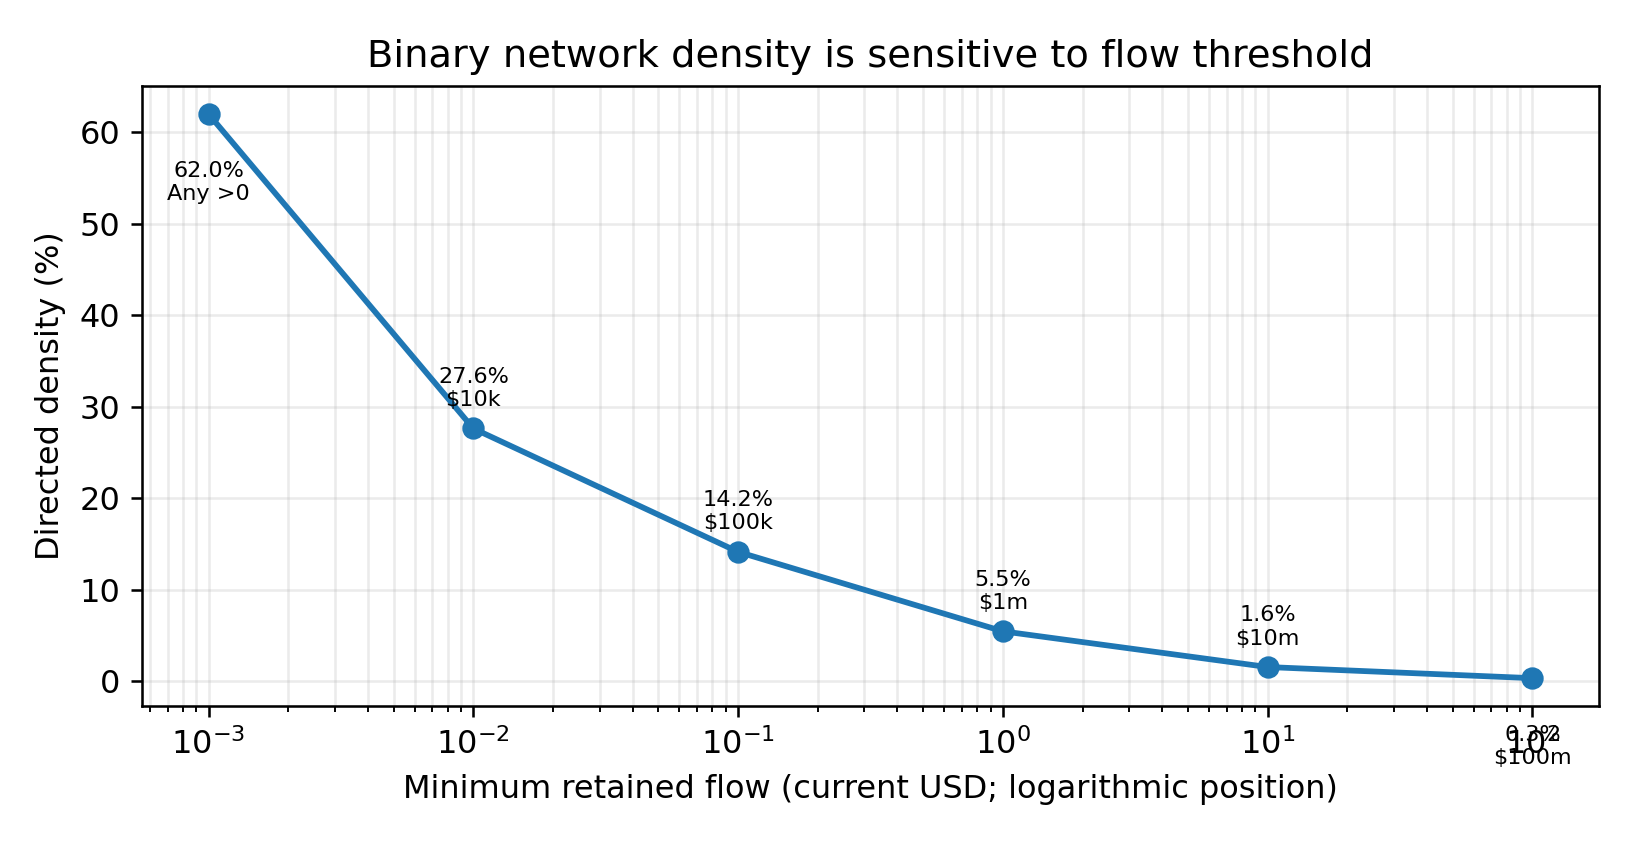
\includegraphics[width=\columnwidth]{edge_threshold_sensitivity.png}
\caption{Directed density falls substantially as the minimum monetary flow required for an edge increases. The first point includes every positive off-diagonal flow.}
\label{fig:threshold-density}
\end{figure}

The total positive intermediate-flow value including self-flows is USD 103.41 trillion; off-diagonal flows total USD 81.13 trillion. Exact self-flows account for 21.55\% of the positive flow total and are excluded from graph connectivity measures. The out-strength and in-strength Gini coefficients are 0.863 and 0.852, respectively, indicating that monetary flows are concentrated among a subset of nodes.

The top out-strength node in the full graph is \texttt{USA\_M}, professional, scientific, and technical activities in the United States, with approximately USD 2.196 trillion in off-diagonal intermediate flows supplied. It is followed by U.S. trade (USD 1.971 trillion) and Chinese trade (USD 1.803 trillion). The highest in-strength node is Chinese construction (USD 3.263 trillion in intermediate inputs purchased), followed by U.S. trade (USD 2.058 trillion). A high out-strength measures supplied monetary flow; a high in-strength measures purchased inputs. Neither measure is equivalent to exports, GDP, or a direct prediction of failure impact.

\begin{figure}[t]
\centering
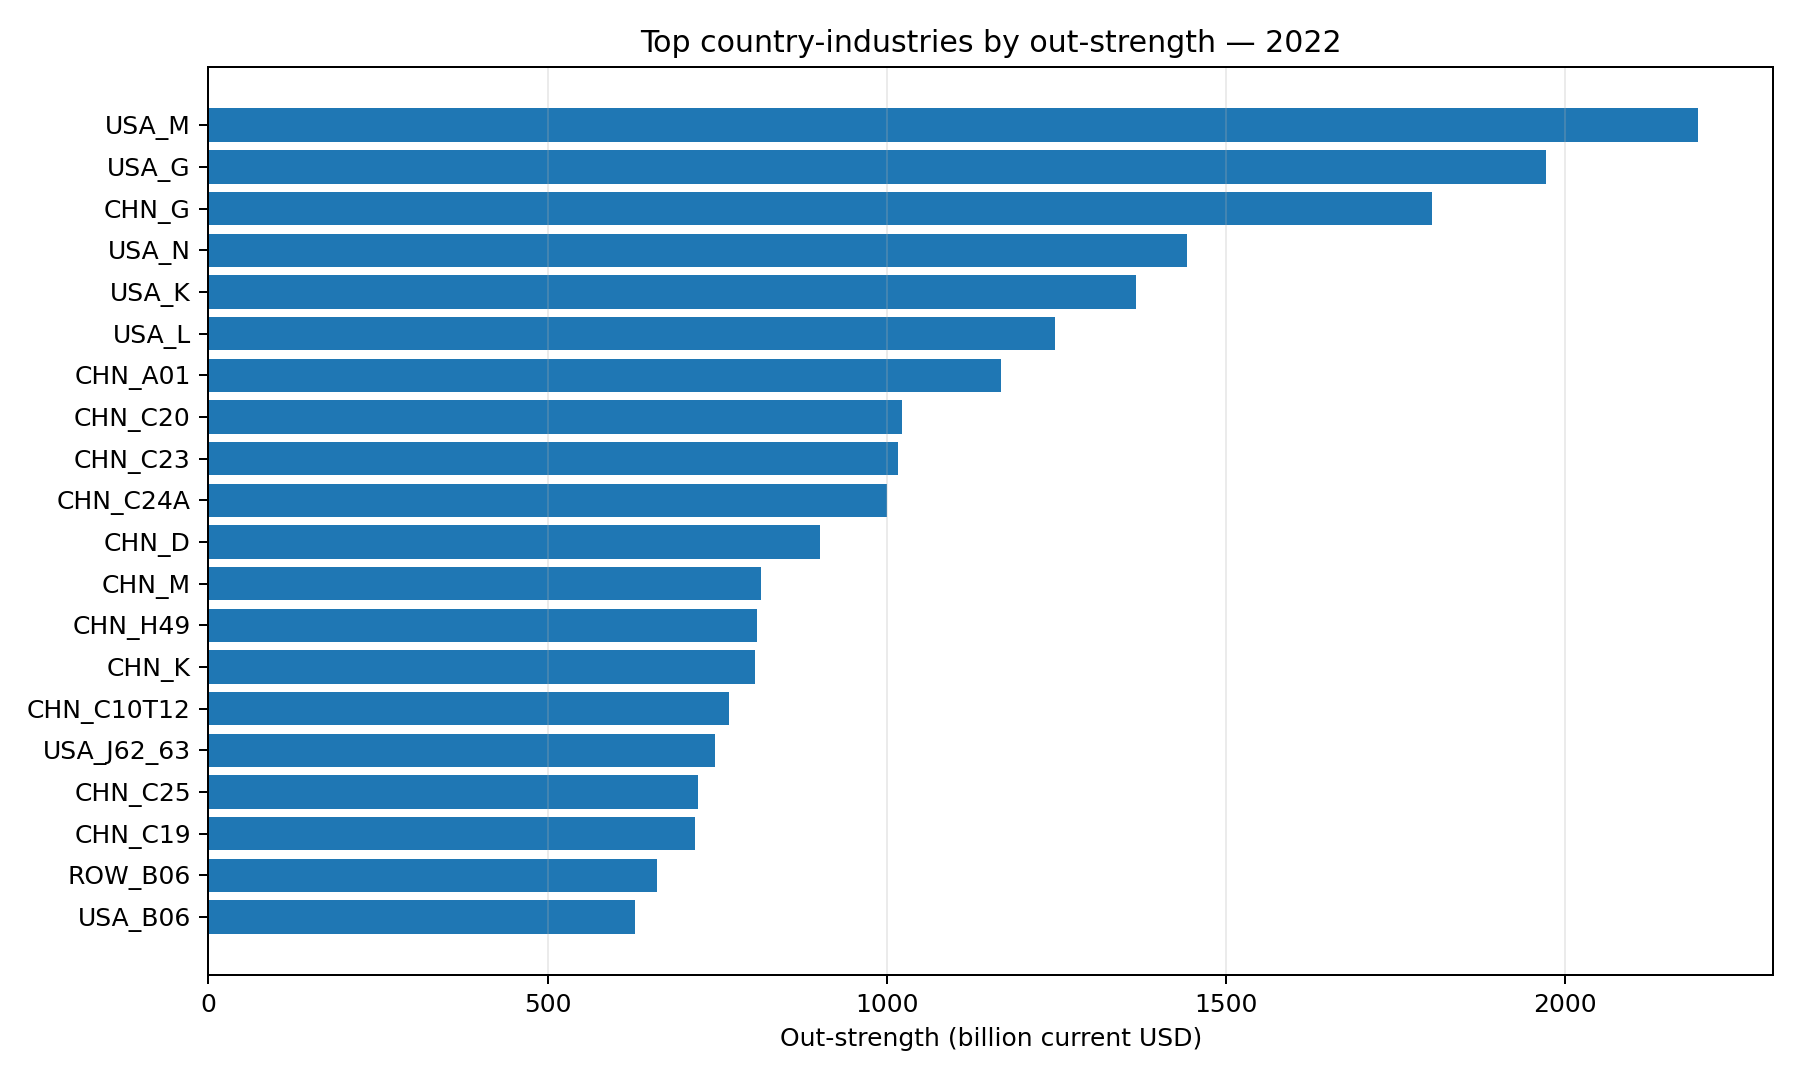
\includegraphics[width=\columnwidth]{top_out_strength.png}
\caption{Top 20 country--industry nodes by off-diagonal out-strength in the full 2022 network, derived from the CSV. Flow values are in billions of current U.S. dollars.}
\label{fig:outstrength}
\end{figure}

Rank correlations on all 4,050 raw nodes show that out-degree and out-strength are positively associated ($\rho=0.764$); in-degree and in-strength are even more closely associated ($\rho=0.945$). Out-strength correlates with weighted PageRank ($\rho=0.799$) and gross output ($\rho=0.909$). These associations are descriptive, not causal. They also indicate that degree counts and monetary size overlap but are not interchangeable.

The sector aggregation gives a second view of the data. Summed across countries, the metals/machinery/electronics/transport group has the largest out-strength (about USD 11.88 trillion) and in-strength (USD 14.72 trillion). Chemicals/petroleum/minerals supplies about USD 10.46 trillion, while professional/administrative services supplies about USD 9.98 trillion. Construction and public/social/other services have comparatively large input purchases (USD 7.98 trillion and USD 8.39 trillion, respectively). These are gross intermediate-flow totals across all regions, not net trade or value added.

\begin{figure*}[t]
\centering
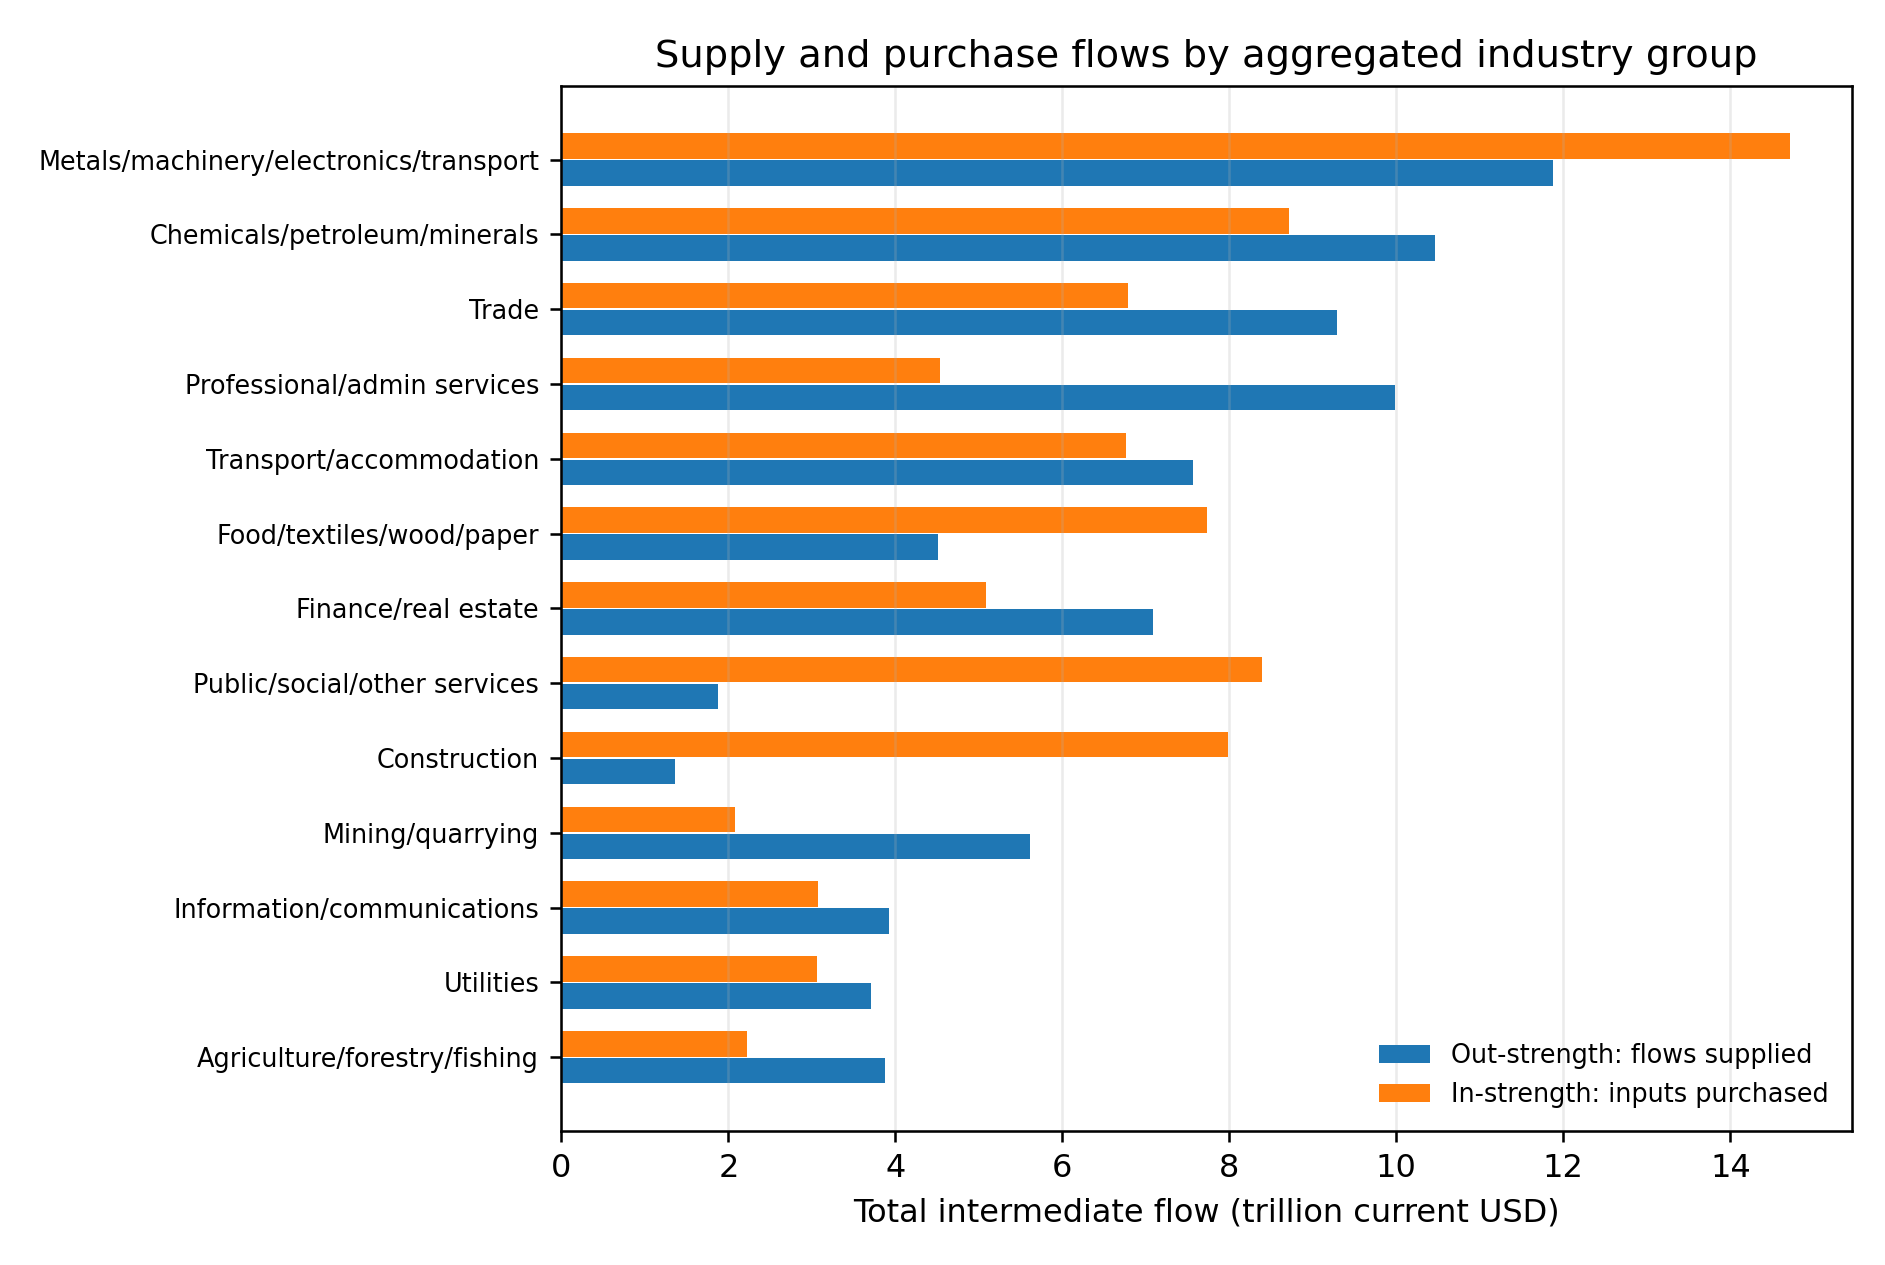
\includegraphics[width=0.93\textwidth]{sector_group_flow.png}
\caption{Total intermediate-flow strengths for the 13 aggregated sector groups, summed across all economies. Out-strength is supplied flows; in-strength is purchased inputs. Values are in trillion current U.S. dollars and exclude exact raw-node self-flows.}
\label{fig:sector-flow}
\end{figure*}

\begin{table}[t]
\caption{Examples of High-Strength Nodes in the Full Network}
\label{tab:topnodes}
\centering
\footnotesize
\begin{tabular}{lrlr}
\toprule
\multicolumn{2}{c}{Out-strength} & \multicolumn{2}{c}{In-strength}\\
Node & USD B & Node & USD B\\
\midrule
USA\_M & 2,196.2 & CHN\_F & 3,263.5\\
USA\_G & 1,971.3 & USA\_G & 2,058.0\\
CHN\_G & 1,803.4 & USA\_O & 1,311.1\\
USA\_N & 1,442.3 & CHN\_C10T12 & 1,253.4\\
USA\_K & 1,366.6 & USA\_L & 1,201.3\\
\bottomrule
\end{tabular}
\end{table}

\section{Dynamical Results}
\subsection{SIS model comparison}
For the highest out-strength seed in the 1,053-node aggregate network (\texttt{USA\_Professional-admin services}), we compare unweighted and dependency-weighted SIS. Table~\ref{tab:sis} reports mean peak $H(t)$ and its standard deviation across 100 runs, along with cumulative disrupted share $C$. When $\beta/\beta_c=1.4$, weighted SIS gives a mean peak of 10.96\% (SD 8.24\%), compared with 5.15\% (SD 4.93\%) for unweighted SIS. The weighted cumulative measure is 1.894 share-steps, compared with 0.425 for the unweighted baseline. The high standard deviations show that outbreak trajectories remain stochastic and variable; the mean should not be read as a deterministic prediction.

At $\beta/\beta_c=0.7$ and 1.0, the weighted model also produces greater average peak and cumulative disruption in these experiments. This does not establish that weighted SIS is more accurate, because no observed outage series is available for validation. Rather, it shows that replacing equal link influences with the observed input-flow scale changes the model's behaviour on this network.

\begin{figure}[t]
\centering
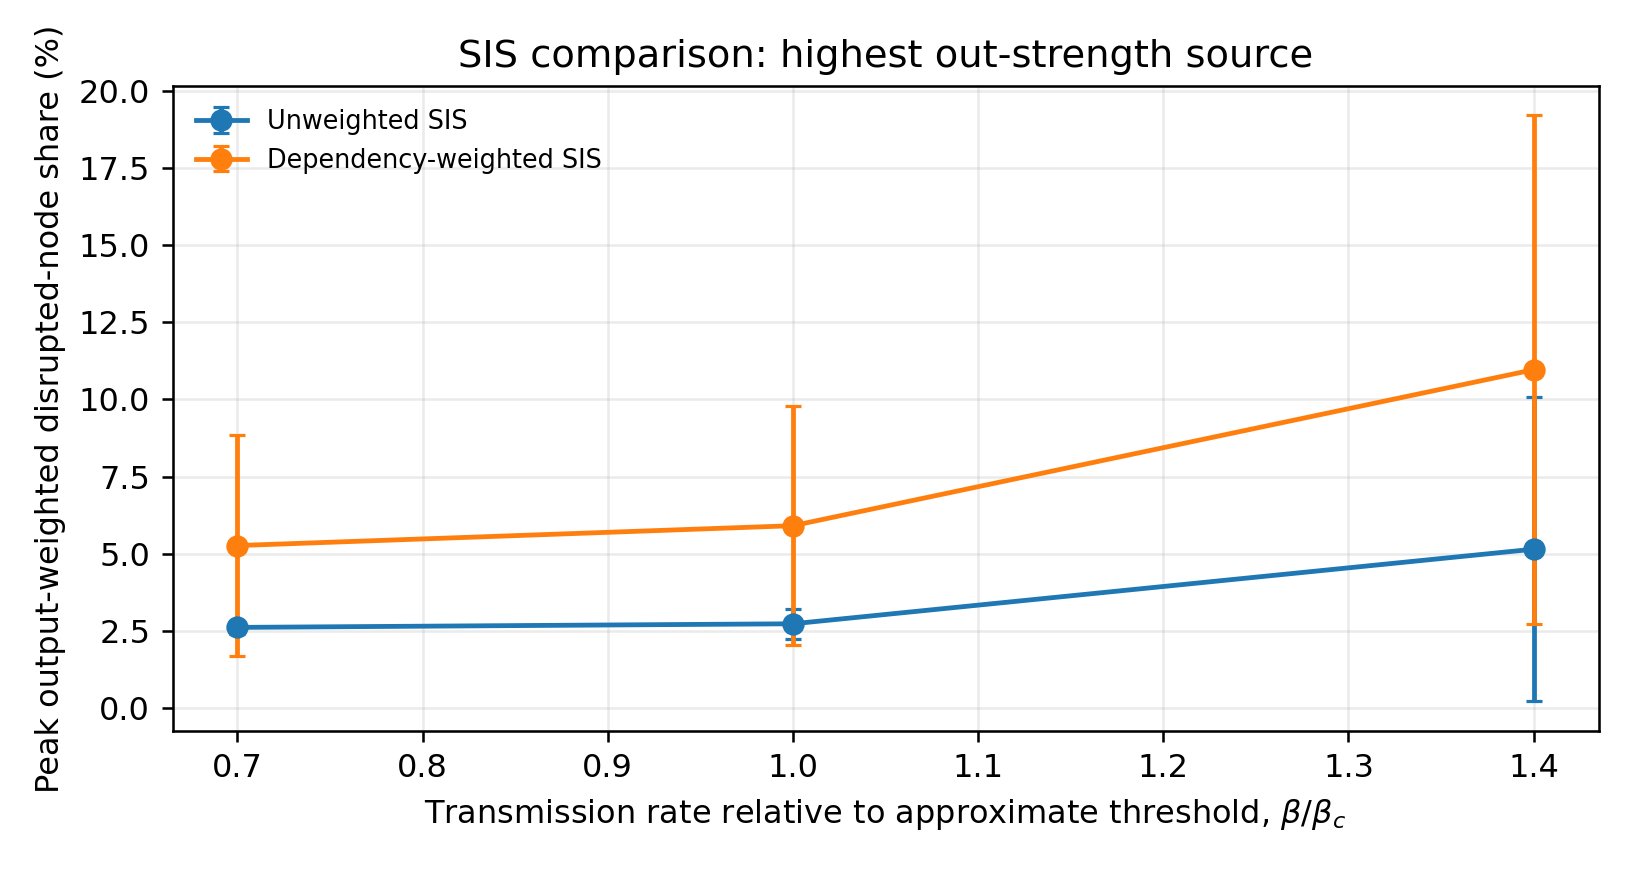
\includegraphics[width=\columnwidth]{sis_model_comparison.png}
\caption{Peak output-weighted disrupted-node share for the highest out-strength source. Error bars show one standard deviation across 100 Monte Carlo runs; large spread is visible at the highest transmission setting.}
\label{fig:sis}
\end{figure}

\begin{table}[t]
\caption{SIS Results for the Highest Out-Strength Seed (100 Runs)}
\label{tab:sis}
\centering
\footnotesize
\begin{tabular}{ccccc}
\toprule
$\beta/\beta_c$ & Unweighted peak (\%) & Weighted peak (\%) & $C_U$ & $C_W$\\
\midrule
0.7 & $2.61\pm0.21$ & $5.26\pm3.57$ & 0.101 & 0.355\\
1.0 & $2.73\pm0.48$ & $5.91\pm3.87$ & 0.143 & 0.485\\
1.4 & $5.15\pm4.93$ & $10.96\pm8.24$ & 0.425 & 1.894\\
\bottomrule
\end{tabular}
\end{table}

In an exploratory source-ranking experiment, we select 65 candidate nodes from the union of top-ranked nodes under five structural/output measures plus random active nodes. Each candidate receives six weighted-SIS runs at $1.4\beta_c$. Spearman correlation between source out-strength and mean peak $H(t)$ is $\rho=0.911$; PageRank versus peak impact gives $\rho=0.871$; out-degree versus peak impact gives $\rho=0.307$. Because the candidate set deliberately over-samples high-ranking nodes, these correlations are exploratory and selection-biased, not population-wide estimates. The result nevertheless motivates testing monetary flow measures rather than assuming simple degree is the best risk proxy.

\subsection{Threshold-cascade sensitivity}
The deterministic threshold model produces a sharp change in outcomes when $\theta$ changes. From the high out-strength source, thresholds of 0.02, 0.05, and 0.10 lead to 1,052 of 1,053 aggregate nodes failing, with an output-weighted failed-node share of 100\%. At $\theta=0.15$, 78 nodes fail and the weighted share falls to 26.52\%; at $\theta=0.30$ or higher, only the seed node fails (2.56\% of summed gross output represented by failed nodes). The high PageRank seed also produces near-total cascades at lower thresholds, but smaller cascades at 0.15 and 0.20.

\begin{figure}[t]
\centering
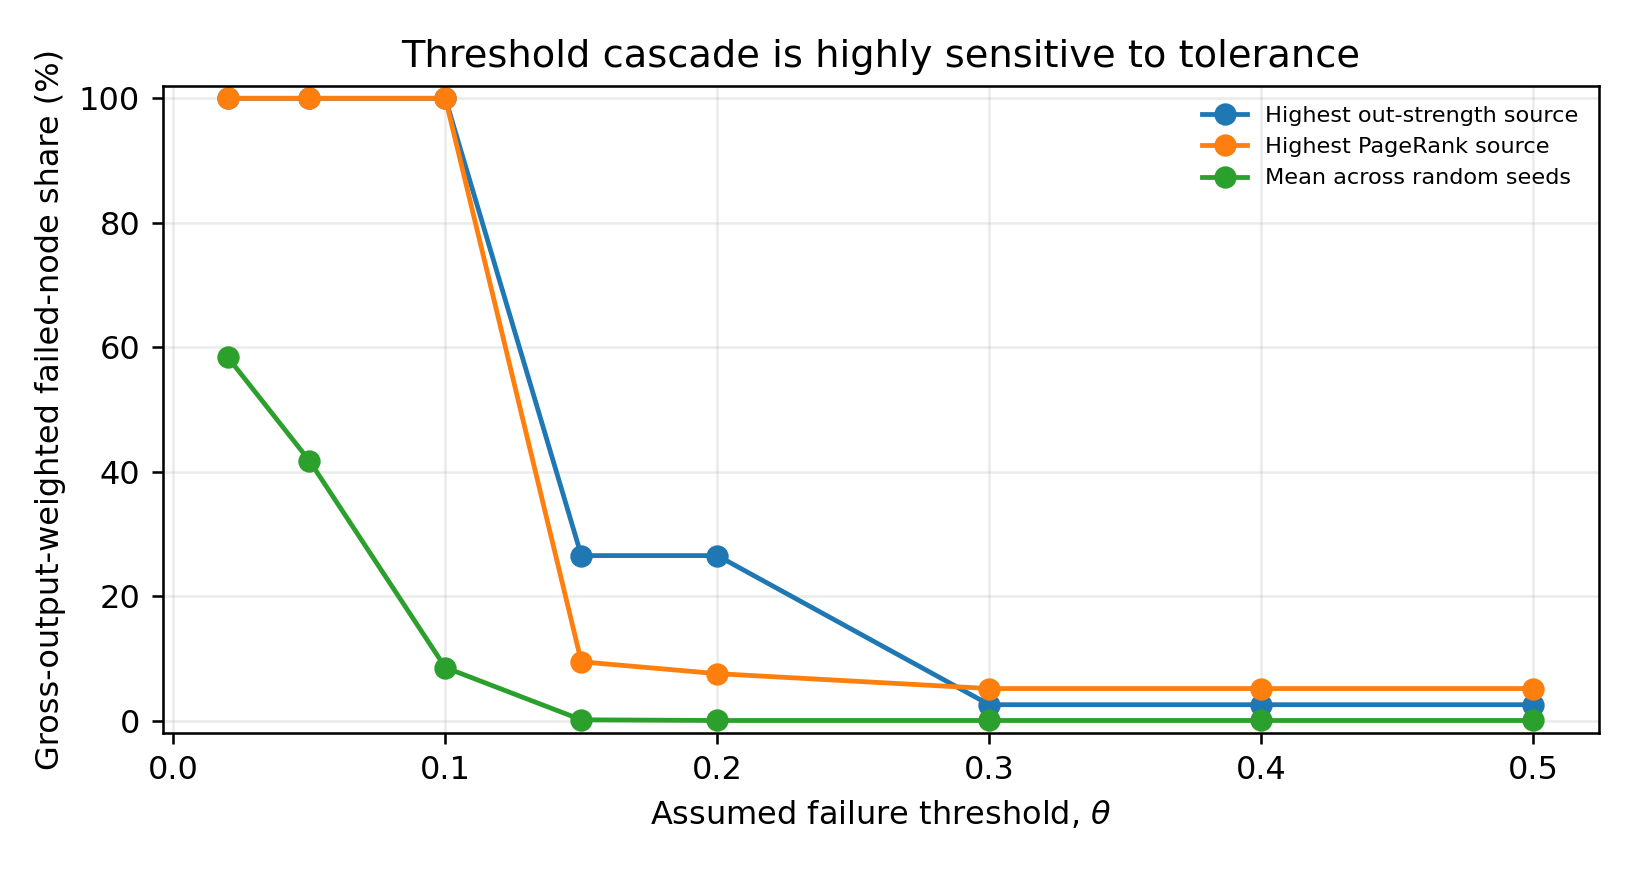
\includegraphics[width=\columnwidth]{threshold_cascade_sensitivity.png}
\caption{Output-weighted failed-node share versus assumed threshold. The sharp transition is a property of this threshold rule and the tested parameters; tolerance thresholds are not identified by ICIO data.}
\label{fig:cascade}
\end{figure}

This experiment demonstrates sensitivity to assumed tolerance. It should not be interpreted as evidence that a real 10\% supplier exposure would collapse the global economy. The IO table supplies the dependency structure, but it does not report inventories, substitutability, safety stock, or sector-specific failure thresholds. The main result is methodological: cascade predictions are highly conditional on these assumptions.

\subsection{Equal-budget protection}
Table~\ref{tab:intervention} compares strategies under 100 paired Monte Carlo runs. Without protection, mean peak $H(t)$ is 11.64\% and mean cumulative $C$ is 2.016 share-steps. Protecting 105 high out-strength nodes reduces the mean peak to 7.37\% and cumulative $C$ to 0.835. High-PageRank protection gives a similar result (7.49\% peak and 0.881 cumulative), while random protection gives 10.66\% peak and 1.737 cumulative.

The paired contrast analysis below quantifies the differences between these strategies. Because the intervention halves outgoing transmission weights and uses a fixed source, its results are conditional on those modelling choices.

\begin{figure}[t]
\centering
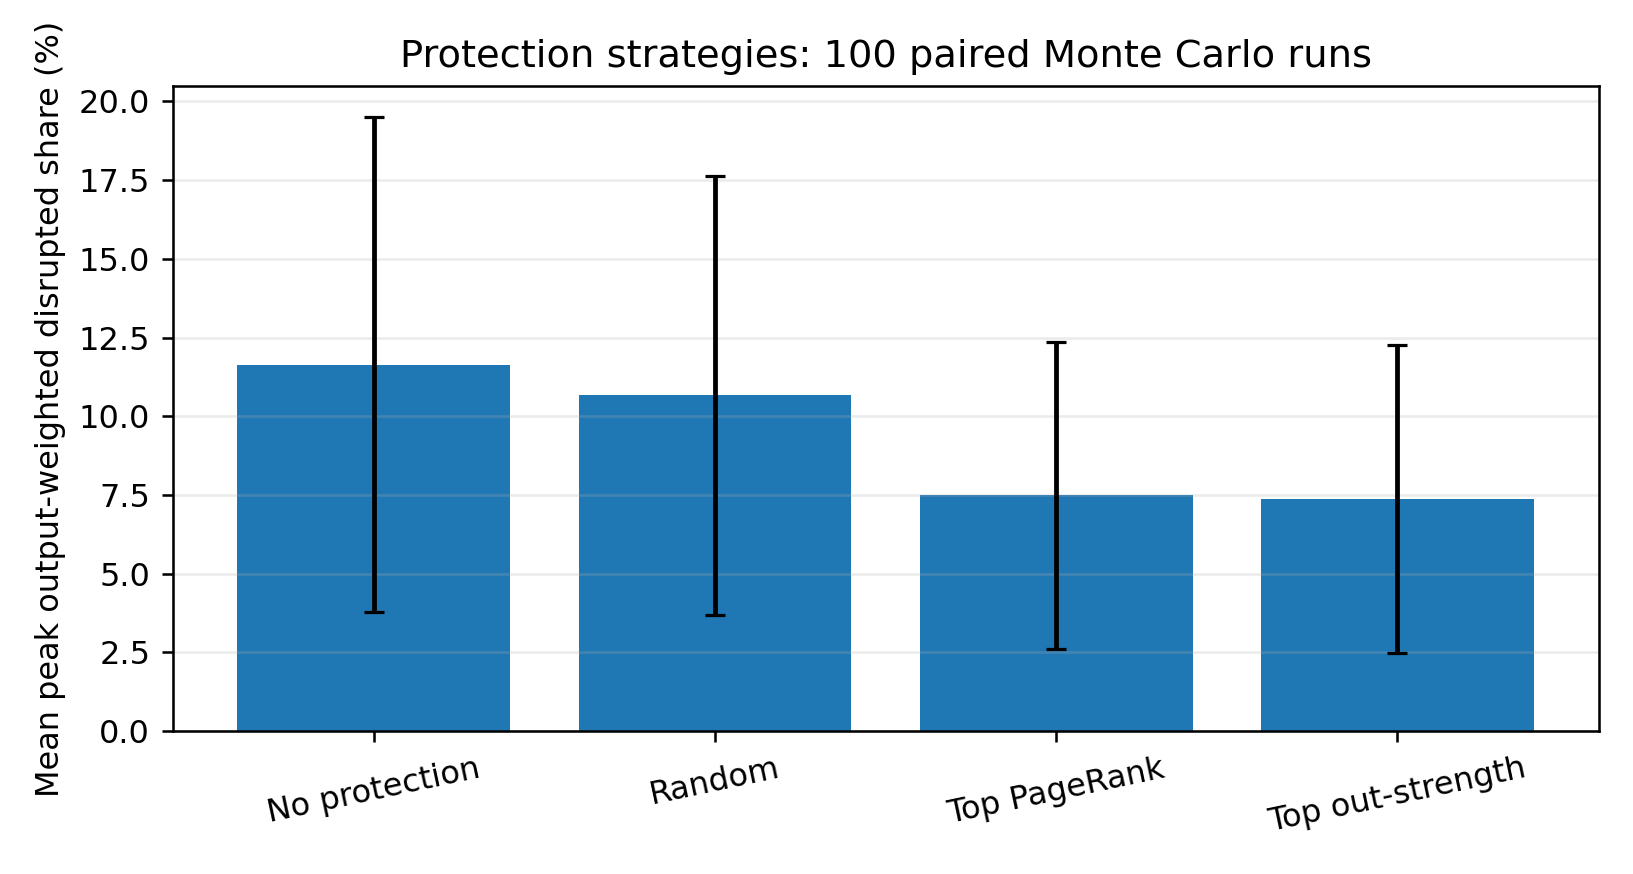
\includegraphics[width=\columnwidth]{intervention_comparison.png}
\caption{Mean peak output-weighted disrupted-node share for no protection and three equal-budget strategies. Error bars show standard deviation across 100 paired Monte Carlo runs.}
\label{fig:intervention}
\end{figure}

\begin{table}[t]
\caption{Equal-Budget Protection Results (100 Paired Runs)}
\label{tab:intervention}
\centering
\footnotesize
\begin{tabular}{lccc}
\toprule
Strategy & Peak $H$ (\%) & Cumulative $C$ & Final $H$ (\%)\\
\midrule
None & $11.64\pm7.87$ & $2.016\pm1.691$ & 5.43\\
Random & $10.66\pm6.97$ & $1.737\pm1.487$ & 4.10\\
Top PageRank & $7.49\pm4.87$ & $0.881\pm0.845$ & 1.29\\
Top out-strength & $7.37\pm4.89$ & $0.835\pm0.818$ & 1.12\\
\bottomrule
\end{tabular}
\end{table}

\subsection{Paired intervention contrasts}
Because the same random-number stream is used for each strategy within a replicate, intervention differences can be compared using paired Monte Carlo contrasts rather than treating each strategy as an unrelated simulation sample. Relative to no protection, out-strength protection reduced the mean peak $H(t)$ by 4.27 percentage points (paired 95\% confidence interval: 3.18--5.37); PageRank protection reduced it by 4.15 points (3.09--5.21); random protection reduced it by 0.98 points (0.51--1.45). The corresponding mean reductions in cumulative $C$ were 1.181 share-steps (95\% CI: 0.943--1.419), 1.135 (0.905--1.365), and 0.279 (0.198--0.361), respectively. These intervals quantify variability in the specified stochastic simulation under common random numbers. They do not represent sampling uncertainty about real-world economic losses. The closeness of the two targeted strategies also suggests that the experiment does not establish a universal superiority of one centrality measure; that ranking could change with the source node, intervention rule, transmission rate, or aggregation scheme.

\section{Discussion and Limitations}
The full ICIO matrix is highly connected when every positive flow counts as an edge, but this topology changes substantially under monetary cutoffs. This suggests that raw binary degree is not enough to describe economic dependence. Weighted flow measures are more interpretable for the question we ask, although current-price flow values still reflect scale and price levels, not just physical criticality.

Three limitations matter. First, the data are annual and contain no time-stamped disruption episodes. Transmission rates, recovery probabilities, and thresholds are therefore assumptions rather than estimates. Second, our output-weighted infection measure uses gross output as a node weight; it marks the share of gross output represented by disrupted nodes, not actual lost output. The summed gross output denominator is not GDP because intermediate goods can be counted at multiple production stages. Third, aggregation to 13 sector groups reduces complexity but conceals differences within broad sectors. The raw network density is also sensitive to tiny positive flows, as shown in Fig.~\ref{fig:threshold-density}.

These limitations define appropriate claims. The simulations can compare alternative assumptions and prioritisation rules on a real economic network, but cannot predict actual losses or prove that the chosen strategy would work in a real crisis. A future extension would calibrate recovery and substitution using documented outage cases, test multiple years after adjusting for nominal-price changes, and compare the dynamical stress tests with OECD direct/indirect value-chain exposure indicators.

\section{Conclusion}
We constructed and analysed the 2022 OECD country--industry production network and used it to test three forms of disruption modelling. Structurally, flows are concentrated and the apparent binary density depends strongly on the edge threshold. In the SIS stress test, the dependency-weighted model produces higher disruption shares than the unweighted baseline for the tested high-out-strength source and transmission settings. The threshold model exhibits abrupt, highly parameter-sensitive cascades. Under the chosen equal-budget intervention rule, protecting nodes with high out-strength or PageRank reduces simulated disruption more than random protection. These results support using weighted network structure and explicit sensitivity analysis in supply-chain stress testing, while underscoring that modeled disruption is not the same as observed economic loss.

\begin{thebibliography}{00}
\bibitem{OECD} OECD, ``Inter-Country Input-Output Tables,'' OECD Data, 2025 edition, revised Jan. 2026. [Online]. Available: \url{https://www.oecd.org/en/data/datasets/inter-country-input-output-tables.html}. Accessed: Oct. 26, 2026.
\bibitem{Acemoglu} D. Acemoglu, V. M. Carvalho, A. Ozdaglar, and A. Tahbaz-Salehi, ``The network origins of aggregate fluctuations,'' \emph{Econometrica}, vol. 80, no. 5, pp. 1977--2016, 2012, doi: 10.3982/ECTA9623.
\bibitem{Berger} N. Berger, S. Schulze-Schwering, E. Long, and S. Spinler, ``Risk management of supply chain disruptions: An epidemic modeling approach,'' \emph{European Journal of Operational Research}, vol. 304, no. 3, pp. 1036--1051, 2023.
\bibitem{Pastor} R. Pastor-Satorras, C. Castellano, P. Van Mieghem, and A. Vespignani, ``Epidemic processes in complex networks,'' \emph{Reviews of Modern Physics}, vol. 87, p. 925, 2015, doi: 10.1103/RevModPhys.87.925.
\bibitem{Watts} D. J. Watts, ``A simple model of global cascades on random networks,'' \emph{Proceedings of the National Academy of Sciences}, vol. 99, no. 9, pp. 5766--5771, 2002, doi: 10.1073/pnas.082090499.
\end{thebibliography}
\end{document}
